\documentclass{ctuthesis}

\ctusetup{
    xdoctype = B,
    xfaculty = F3,
    mainlanguage = czech,
    secondlanguage = english,
    titlelanguage = czech,
    title-english = {UI toolkit of accessible web components},
    title-czech = {UI toolkit přístupných webových komponent},
    department-czech = {Katedra počítačové grafiky a interakce},
    department-english = {Department of Computer Graphics and Interaction},
    fieldofstudy-czech = {Softwarové inženýrství a technologie},
    subfieldofstudy-czech = {Programátor / architekt webových aplikací},
    keywords-czech={Web komponenty, přístupnost, WAI-ARIA, WCAG, APG, Solid.js},
    keywords-english={Web components, accessibility, WAI-ARIA, WCAG, APG, Solid.js},
    author = {Pavel Sušický},
    supervisor = {Bc. Petr Huřťák},
    month = 5,
    year = 2024,
    specification-file={./assets/documents/zadani.pdf},
    front-specification={true}
}

\usepackage{csquotes}

\usepackage[style=iso-numeric,backend=biber,sorting=none,alldates=short,block=ragged]{biblatex}

\addbibresource{thesis.bib}

\usepackage[style=altlist]{glossaries}

\makenoidxglossaries{}

\newacronym{wcag}{WCAG}{Web Content Accessibility Guidelines}
\newacronym{waiaria}{WAI-ARIA}{Web Accessibility Initiative --- Accessible Rich Internet Applications}
\newacronym{apg}{APG}{ARIA Authoring Practices Guide}
\newacronym{w3c}{W3C}{World Wide Web Consortium}
\newacronym{wai}{WAI}{Web Accessibility Initiative}

\newacronym{dom}{DOM}{Document Object Model}
\newacronym{vdom}{VDOM}{Virtual DOM}

\newglossaryentry{lighthouse}{
    name={Ligthouse},
    description={Lighthouse je nástroj od Google pro provádění auditu stránky z různých hledisek. V kontextu této práce je využivána ``Time To Interactive'' metrika a velikost přenesených dat},
}

\newglossaryentry{todomvc}{
    name={TodoMVC},
    description={TodoMVC je kolekce příkladové aplikace implementované v různých webových technologiích},
}

\usepackage{xcolor,listings,chngcntr,etoolbox}

\makeatletter
\patchcmd{\@chapter}% <cmd>
{\addtocontents}% <search>
{\addtocontents{lol}{\protect\addvspace{10\p@}}% Add per-chapter space in LoL
    \addtocontents}% <replace>
{}{}% <success><failure>
\makeatother

% NOTE: Add space before minted environment
\BeforeBeginEnvironment{minted}{\bigskip}

% NOTE: Define a new command for labeling inside minted environment
\newcommand{\mintedlabel}[1]{\phantomsection\label{\detokenize{#1}}}

% NOTE: Set the format of the listing caption
\counterwithin{listing}{chapter}
\renewcommand{\thelisting}{\thechapter.\arabic{listing}}

% NOTE: Setup minted
\setminted{
    linenos,
    escapeinside=!!
}

\renewcommand\listingscaption{Ukázka kódu}
\renewcommand\listoflistingscaption{Ukázky kódu}
\renewcommand{\baselinestretch}{1.25}

\definecolor{codegreen}{rgb}{0,0.6,0}
\definecolor{codegray}{rgb}{0.5,0.5,0.5}
\definecolor{codepurple}{rgb}{0.58,0,0.82}
\definecolor{backcolour}{rgb}{0.99,0.99,0.99}
\definecolor{black}{rgb}{0,0,0}

\usepackage{tabularx,array}

\newcolumntype{Y}{>{\centering\arraybackslash}X}

\definecolor{OK}{RGB}{0, 128, 0}
\definecolor{NOT_OK}{RGB}{128, 0, 0}

\newcommand{\fr}[1]{\texttt{\textbf{#1}}}


\ctuprocess{}

\begin{thanks}
    Chtěl bych zde poděkovat svému vedoucímu práce Bc. Petrovi Huřťákovi za cenné rady a pomoc při tvorbě této práce.

    Dále bych chtěl vyjádřit obrovské poděkování mé rodině a to hlavně mé mamince Pavlíně za veškerou podporu při mém studiu.

    Stejně velký vděk patří i mému tatínkovi Jiřímu za jeho cenné rady a zkušenosti, které mi pomáhají v dennodenním životě.

    V neposlední řadě i mým bratrům Honzovi a Kubovi, kteří si pro mě vždy našli čas a pomohli mi s čímkoliv, co jsem potřeboval.
\end{thanks}

\begin{declaration}
    Prohlašuji, že jsem předloženou práci vypracoval samostatně a že jsem uvedl veškeré použité informační zdroje v souladu s Metodickým pokynem o dodržování etických principů při přípravě vysokoškolských závěrečných prací.
    \\ \\
    V Praze dne TODO

    \vspace{15mm}
    \begin{tabular}{@{}p{2.5in}@{}}
    \hrulefill{} \\
    \centerline{Pavel Sušický}
    \end{tabular}
\end{declaration}

\begin{abstract-english}
The bachelor thesis deals with the issue of reusable components in the context of UI creation for websites and web applications.
The thesis aims to implement components from a collection of design patterns published by the informative resource Aria Authoring Practices in the Solid.js framework.
The work includes analysis of existing solutions across the JavaScript ecosystem and testing the implemented components.
The work yields components and documentation describing their use. These components are distributed within the ecosystem for other developers to use for their projects.
\end{abstract-english}

\begin{abstract-czech}
Bakalářská práce se zabývá problematikou znovupoužitelných komponent v kontextu tvorby rozhraní pro webové stránky a aplikace.
Cílem práce je implementovat komponenty z kolekce návrhových vzorů publikované informativním zdrojem Aria Authoring Practises ve frameworku Solid.js.
Součástí práce je i analýza existujících řešení napříč vývojářským ekosystémem a testování implementovaných komponent.
Výsledkem práce jsou komponenty a dokumentace pro jejich použití, tyto komponenty jsou distribuovány v rámci ekosystému pro další vývojáře, kteří je mohou využít pro své projekty.
\end{abstract-czech}

\begin{document}

\maketitle

\chapter{Úvod}

Přístupnost na webu je v dnešní době důležitá. Tato práce se zabývá implementací JavaScriptové knihovny
znovupoužitelných, nestylovaných (low-level) komponent, které jsou implementované podle moderních specifikací publikovaných konsorciem W3C.

V teoretické části se věnuji problematice přístupnosti na webu, kde popisuji účel existence
Web Accessibility Initiative --- Accessible Rich Internet Applications (dále jen \textbf{WAI-ARIA}).
Součástí této kapitoly je analýza existujících doporučení pro tvorbu webových
komponent pod názvem ARIA Authoring Practices Guide (dále jen \textbf{APG}) a
obecných doporučení pro přístupný web Web Content Accessibility Guidelines (dále jen \textbf{WCAG}).

V praktické části práce se zabývám implementací knihovny komponent,
které jsou přístupné, tedy jsou implementované podle doporučení od WAI-ARIA.

\section{Motivace}

V současné době jsou znovupoužitelné komponenty nejčastějším způsobem jakým se vytváří webové aplikace, protože většina knihoven (například React, Vue, Angular, SolidJS a další) využívají komponentové paradigma.

Vznik komponent tak vedl k vytvoření souboru komponent tzv.\ component libraries obsahující základní prvky, které denně potkáváme na internetu, aby je vývojář nemusel znovu implementovat pro každou aplikaci zvlášť.

Vývoj znovupoužitelných komponent je však náročný, protože kromě implementačních detailů je nutné se zabývat i přístupové problematice. Toto vedlo k nekonzistenci napříč knihovnami, kde nejvíce používané knihovny (React, Vue, \dots) takové knihovny komponent mají, ale méně používané knihovny (Svelte, SolidJS, Lit) takové knihovny nemají, nebo jejich kvalita je nízká.

\section{Cíl práce}


Hlavním výsledkem této práce by měla být knihovna, která rozšíří ekosystém frameworku Svelte o znovupoužitelné, stylovatelné a přístupné komponenty.


\begin{figure}
    \centering
    \includegraphics[width=0.5\textwidth]{./assets/figures/chapter-1/otter.jpg}
    \caption{Otters are awesome!}
\end{figure}


\part{Relevantní technologie}

\chapter{Technologie a metodiky přístupnosti na webu}

V této kapitole se věnuji představení problematice přístupnosti na webu.

\section{Přístupný web}

Přístupnost na webu je definována jako schopnost webového obsahu být interpretován a používán nejširším možným spektrem uživatelů bez ohledu na jejich schopnosti, nebo fyzický stav~\cite{w3-accessibility}.

\section{Základní principy přístupnosti}

V této sekci popisuji základní principy přístupnosti, které jsou relevantní v kontextu této práce, tedy vytváření znovpoužitelných komponent. Existují avšak i další principy, které se obecně zaměřují na webový obsah, porozumění textu anebo přístupnost audiovizuálního obsahu~\cite{w3-accessibility-principles}.

\subsection{Ovládání pomocí klávesnice}

\section{Web accessibility initiative}

\section{Accessible Rich Internet Applications}

\section{Web content accessibility guidelines}

\section{Aria authoring practices guide}

% \section{Čtečky obrazovky}

\chapter{Technologie}

Tato kapitola představuje důležité technologie a přístupy použité v rámci této práce.

\section{Solid.js}

\fr{Solid.js}\footnote{\url{https://solidjs.com}} je JavaScriptová knihovna pro tvorbu uživatelských rozhraní obdobně jako React, Vue, nebo Svelte.


\subsection{Rozdíly}

Rozdíl mezi Solid.js a ostatními knihovnami spočívá v technologii synchronizování změn v \gls{dom}.

Populární knihovny jako React, nebo Vue používají tzv. \gls{vdom}, což je virtuální reprezentace \gls{dom} stromu v paměti, která se porovnává s reálným \gls{dom} stromem a rozdíly mezi nimi se aplikují pomocí \textit{diffing} algoritmu.

Solid.js a nově i Svelte používají granulární, reaktivní modely pro sledování změn v \gls{dom}.
Prakticky Solid.js využívá principu \textit{dependency tracking}, kde přístupy k reaktivním proměnným jsou sledovány skrze \textit{subscribers}, kteří jsou upozornění na případné změny respektive zápisy do těchto proměnných~\cite{solid-reactivity}.
Tento princip připomíná designový vzor \textit{observer}.

\subsection{Rychlost}

Tabulka~\ref{tab:technology1} porovnává Solid.js s vybranými \textit{frameworky}.
Všechny metriky jsou vypočítané na příkladové aplikaci \fr{\gls{todomvc}}\footnote{\url{https://todomvc.com}} implementované v daném frameworku, aby test byl spravedlivý.
Každé skóre je číslo normalizované do intervalu <1, $\infty$), které nám říká velikost zhoršení oproti nejlepší implementaci~\cite{krausest120,krausest122}.

První metrika ``Operations'' je vážený geometrický průměr skóre všech operací nad příkladovou aplikací (např. vytvoření řádku, smazání řádku, vybraní řádku a další\dots).

Druhá metrika ``Transferred size'' je vážený geometrický průměr skóre přenesených dat po síti při použití daného frameworku.

Poslední metrika ``Memory allocation'' je vážený geometrický průměr skóre využití paměti.

% % TODO: Different background color for table

\begin{table}[ht]
      \begin{ctucolortab}
            \begin{tabular}{c c c c c}
                  \bfseries Metrika & \bfseries{Solid 1.8.0} & \bfseries{Svelte 5} & \bfseries{Vue 3.3.6} & \bfseries{React 18.2.0} \\\Midrule{}
                  Operations        & \textbf{1.08}          & 1.08                & 1.24                 & 1.53                    \\
                  Transferred size  & \textbf{2.29}          & 3.04                & 7.16                 & 15.32                   \\
                  Memory allocation & \textbf{1.45}          & 1.52                & 2.13                 & 2.81
            \end{tabular}
      \end{ctucolortab}
      \captionsetup{justification=centering}
      \caption{Porovnání rychlosti Solid.js s populárními frameworky. \newline Zdroj: Data převzata od Stefana Krause~\cite{krausest120,krausest122}.}
      \label{tab:technology1}
\end{table}

Z výsledku \textit{benchmarku} můžeme vidět, že Solid.js obdobně jako Svelte je velice blízko 1, tedy je jenom o 8\% pomalejší než nejrychlejší implementace.
Svelte od verze 5 má obdobný styl reaktivního modelu jako Solid.js, což vysvětluje podobné výsledky~\cite{svelte-reactivity}.

% \section{Svelte}\label{sec:Svelte}

% Svelte je kompilátor pro tvorbu uživatelských rozhraní obdobně jako populární alternativy React, nebo Vue.
% Každá komponenta se nachází v souboru s příponou ``.svelte'' a podobně jako Vue obsahuje tři části:

% \begin{itemize}
%     \item \textbf{Script tag} --- obsahuje logiku komponenty v JavaScriptu.
%     \item \textbf{Style tag} --- obsahuje styly komponenty.
%     \item \textbf{Template} --- obsahuje html kód komponenty.
% \end{itemize}

% \subsection{Rozdíly}

% Mezi hlavní rozdíly Svelte oproti jiným frameworkům patří:

% \begin{itemize}
%     \item \textbf{Kompilátor} --- Největší rozdíl oproti zmíněným frameworkům se vyskytuje v tom, že Svelte není runtime, který se posíla na klienta společně se zdrojovým kódem komponent.
%           Svelte je kompilátor souborů s příponou ``.svelte'', který převede komponenty na optimalizovaný imperativní kód v JavaScriptu.
%     \item \textbf{Reaktivita} --- Svelte používá reaktivní model pro změny v \gls{dom} namísto \gls{vdom}.
%     \item \textbf{Podpora komunity} --- Svelte není produktem velkých společností jako je React od Meta Platforms, nebo Angular od Google.
%           Zároveň už to není čistě produkt autora Riche Harrise a komunity, ale od roku 2021 je vývoj plně sponzorován platformou Vercel.
%     \item \textbf{Vývojářská přívetivost (DX)} --- Svelte je v praxi jednodušší na používání a intuitivní i pro nové vývojáře.
% \end{itemize}

% Kompilátor s sebou nese jednu nevýhodu a to je velikost výsledného kódu po kompilaci.
% Prázdný projekt ve Svelte má minimální velikost, protože zde není potřeba téměř žádného imperativního kódu pro zaručení reaktivity.
% To vede k tomu, že každá nová komponenta přidává unikátní kus kódu a zvyšuje tak velikost dat, které se posílají přes internet na klienta.
% Existuje tak inflexní bod, kdy velikost aplikace bude vyšší než aplikace napsané v Reactu.
% V praxi se však ukazuje, že toto může být potenciálně problémové pouze u velkých aplikací s velkým počtem komponent~\cite{svelte-scaling}.
% \subsection{VDOM vs Reaktivita}

% Důležitý rozdíl mezi Svelte a podobnými frameworky je ten, že neobsahuje \gls{dom} diffing algoritmus jako to je u Reactu.
% Veškeré změny v \gls{dom} jsou ve Svelte řešené pomocí reaktivních proměnných, které automaticky při své změně vyvolají změnu i ve zmíněném \gls{dom}.
% Sledování změn je zaručeno na základě vytvořeného imperativního kódu při kompilaci (viz. sekce~\ref{sec:Svelte} a ukázky kódu~\ref{svelte-counter} a~\ref{svelte-counter-compiled}).

% \begin{lstlisting}[caption={Počítadlo ve Svelte 4}, label={svelte-counter}, language=html]
% <script>
% 	let count = 0(*@\label{svelte-counter-2}@*)

% 	function add() {
% 		count++
% 	}
% </script>

% <button on:click={add}>+1</button>(*@\label{svelte-counter-9}@*)
% <p>Current count: {count}</p>(*@\label{svelte-counter-10}@*)
% \end{lstlisting}

% V ukázce kódu~\ref{svelte-counter} je důležitá deklarace proměnné \texttt{count} na řádku~\ref{svelte-counter-2}.
% Veškeré změny této proměnné jsou sledovány (viz. ukázka kódu~\ref{svelte-counter-compiled}).
% Na řádku~\ref{svelte-counter-9} je vidět přiřazený callback \texttt{add} na událost click.
% Následně můžeme vidět použití proměnné \texttt{count} na řádku~\ref{svelte-counter-10} v rámci textového uzlu elementu.

% \clearpage

% \begin{lstlisting}[caption={Počítadlo po kompilaci}, label={svelte-counter-compiled}, language=JavaScript]
% function instance($$self, $$props, $$invalidate) {
%     let count = 0;

%     function add() {
%         $$invalidate(0, count++, count);(*@\label{svelte-counter-compiled-5}@*)
%     }

%     return [count, add];
% }

% class App extends SvelteComponent {
%     constructor(options) {
%         super();
%         init(this, options, instance, create_fragment, safe_not_equal, {});
%     }
% }
% \end{lstlisting}

% V zjednodušené ukázce kódu~\ref{svelte-counter-compiled} je na řádku~\ref{svelte-counter-compiled-5} podstatné volání funkce \texttt{\$\$invalidate}, která zaručuje reaktivitu proměnné \texttt{count}.
% Každé přiřazení hodnoty je kompilátorem převedeno na volání funkce \texttt{\$\$invalidate}, které označí danou proměnnou jako změněnou a následně naplánuje její změnu včetně aktualizace elementů, kde se používá.

% \subsection{Rychlost}

% Tabulka~\ref{tab:technology1} ukazuje porovnání Svelte s vybranými frameworky.
% Všechny metriky jsou vypočítané na příkladové aplikaci \gls{todomvc} implementované v daném frameworku, aby test byl spravedlivý.
% Každé skóre je číslo normalizované do intervalu <1, $\infty$), které nám říká velikost zhoršení oproti nejrychlejší implementaci~\cite{krausest119,krausest120}.

% První metrika ``Operations'' je celkový vážený geometrický průměr skóre všech operací nad příkladovou aplikací (např. vytvoření řádku, smazání řádku, vybraní řádku a další\dots).

% Druhá metrika ``Startup metrics'' je vážený geometrický průměr skóre výsledků z \gls{lighthouse} testování.

% Poslední metrika ``Memory allocation'' je vážený geometrický průměr skóre využití paměti.

% % TODO: Different background color for table

% \begin{table}[ht]
%     \begin{ctucolortab}
%         \begin{tabular}{c c c c c}
%             \bfseries Metrika & \bfseries{Svelte 5} & \bfseries{Svelte 4} & \bfseries{Vue 3.3.6} & \bfseries{React 18.2.0} \\\Midrule{}
%             Operations        & 1.06                & \textbf{1.26}       & 1.22                 & 1.43                    \\
%             Startup metrics   & 1.06                & \textbf{1.02}       & 1.27                 & 1.67                    \\
%             Memory allocation & 1.48                & \textbf{1.36}       & 1.86                 & 2.45
%         \end{tabular}
%     \end{ctucolortab}
%     \caption{Porovnání rychlosti Svelte s populárními frameworky}
%     \label{tab:technology1}
% \end{table}

% Z výsledků můžeme vidět, že Svelte 4 je optimalizované velikostně pro start aplikace a využití paměti, což vychází z principu kompilátoru.
% V další kapitole se podívám na to, jak se mění princip Svelte v nové verzi 5, která přináší velké změny v architektuře Svelte.

\section{TypeScript}

JavaScript je dynamicky typovaný jazyk, což se v praxi ukázalo jako těžkopádné při škálování velkých projektů.
Postupem času vznikly různé nástroje a nadstavby nad samotným jazykem, které přidávají statické typování.
Nástroje jako \fr{TypeScript}\footnote{\url{https://typescriptlang.org}}, \fr{Flow}\footnote{\url{https://flow.org}}, nebo \fr{ReasonML}\footnote{\url{https://reasonml.github.io}} se ukázaly jako vhodným řešením pro škálovatelnost, znovupoužitelnost a přehlednost kódu.
Pomyslným vítězem se v posledních letech ukázal TypeScript, který má vysokou popularitu i podporu v rámci ekosystému, proto není náhodou, že ho ve své práci plně používám.
TypeScript dodává znovupoužitelným komponentám větší přehlednost při zpětném čtení kódu, ale i konzumenti komponent mají k dispozici robustní typovou kontrolu včetně fungujícího automatického doplňování kódu.

\section{Distribuce komponent}

\begin{itemize}
      \item \textbf{Knihovna komponent} je taková knihovna komponent, která už má předepsané styly. Většinou je možnost přepsat většinu stylů pomocí ``themes'', ale HTML kód komponent je téměř vždy neměnitelný.
            Hodně se stává, že vývojáři potřebují odlišnou HTML strukturu než je dána.
            Častým případem je právě řešení přístupnosti, kdy je potřeba přidat elementy navíc do komponenty pro např. správné fungování čteček obrazovky.
            \begin{lstlisting}[caption={Ukázka použití komponentové knihovny}, label={component-distribution}, language=html]
import { Button } from "component-library"

export const Dashboard = () => {
      return (
            <div>
                  <Button>Open file</Button>
            </div>
      )
}
\end{lstlisting}
      \item \textbf{Knihovna headless komponent} se liší od klasické knihovny komponent tím, že neobsahuje předepsané styly.
            Zde můžeme rozlišit dvě různé úrovně \textit{headless} komponent.
            \begin{itemize}
                  \item Exportující jednotlivé prvky komponenty, konzument tak má větší kontrolu nad výsledným kódem komponenty.
                        Ovšem HTML struktura v jednotlivých prvcích komponent není stále plně flexibilní.
                  \item Exportující pouze logiku v podobě ``primitiv''. V Reactu se jedná o ``custom hooks'', ve Vue ``composition utilities'', ve Svelte to jsou prosté funkce, které pracují s reaktivními proměnnými a obdobně i ve Solid.js.
            \end{itemize}
      \item \textbf{Copy and paste} není klasická knihovna.
            Tato varianta vznikla jako reakce na headless komponenty a primitiva.
            Jedná se o způsob distribuce komponent, kde konzumenti si zkopírují předpis komponenty.
            Využívá tak existujících headless komponent, nebo UI primitiv.
            Tato varianta je velmi flexibilní, protože umožňuje distributorům přidávat vzorové styly, které konzument může smazat, nebo vyměnit za vlastní řešení.
            Zároveň má konzument plnou kontrolu nad kódem komponenty.
            Nevýhodou je horší znovupoužitelnost a zároveň nutnost manuální aktualizace komponenty pokud se změní její logika.
            Distribuce takových komponent je většinou v podobě \gls{cli}, nebo zkopírováním z dokumentace.
\end{itemize}

\begin{lstlisting}[caption={Ukázka použití headless knihovny}, label={component-distribution-2}, language=html]
import { Tab } from "headless-component-library"

export const Toolbar = () => {
  return (
    <Tab.Group>
      <Tab.List className="flex flex-col gap-4">
        <Tab>
          {({ selected }) => (
            <button
              className={
                selected ? 'bg-blue-500' : 'bg-white'
              }
            >
              Tab 1
            </button>
          )}
        </Tab>
      </Tab.List>
      <Tab.Panels>
        <Tab.Panel>Content 1</Tab.Panel>
      </Tab.Panels>
    </Tab.Group>
  )
}
\end{lstlisting}

V porovnání všech tří přístupů na obrázku~\ref{component-lib-distribution-comparison} můžeme vidět, že vyšší flexibilita přináší i vyšší úroveň abstrakce.
To znamená, že čím flexibilnější je \gls{api} komponenty, tím více času je potřeba pro pochopení, použití a údržbu komponent.

Knihovny komponent jsou nejvýhodnější, pokud není potřeba vlastního \textit{brand}\footnote{Brand designem se rozumí vlastní barvy, fonty, styl ikon a celkově unikátní vizuál.} designu a zároveň jsme spokojení s úrovní přístupnosti, kterou nám komponenta dodává.

Headless komponenty jsou lepší v situacích, kde potřebujeme zasáhnout významně do designu (kaskádových stylů) komponenty pro vlastní potřeby.
Nicméně se tím navyšuje i čas strávený na vývoji.

UI primitiva jsou nejvýhodnější při budování vlastního designového systému, kde potřebujeme plnou kontrolu nad kódem komponenty.

Copy and paste přístup je nejvýhodnější, pokud chceme to nejlepší ze všech přístupů.
Flexibilitu headless komponent případně UI primitiv a zároveň rychlost vývoji jako při použití knihovny komponent.

\begin{figure}[h]
      \centering
      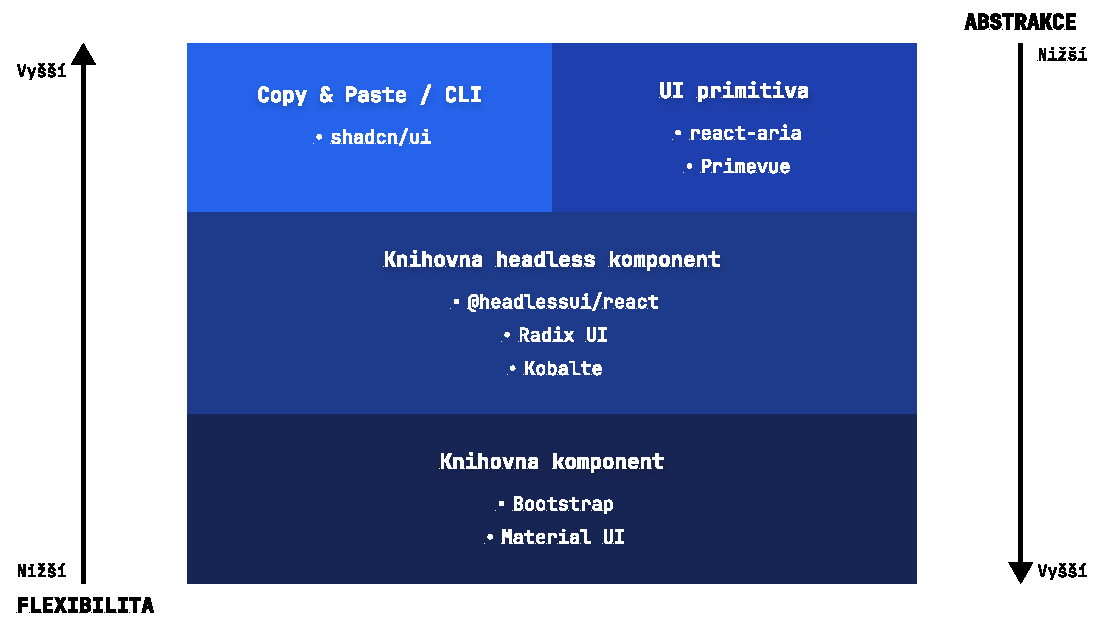
\includegraphics[width=\textwidth]{./assets/figures/component-lib-distribution-comparison.png}
      \captionsetup{justification=centering}
      \caption{Diagram abstrakce a flexibility různých přístupu k distribuci komponent}
      \label{component-lib-distribution-comparison}
\end{figure}

\section{Závěr kapitoly}

Tato kapitola popsala nejdůležitější technologie a přístupy, které jsou využity v rámci této práce.
Plná funkčnost celého projektu je závislá na dalších důležitých technologiích, které zde nejsou popsány neboť nejsou přímo relevantní k problematice tvorby znovupoužitelných komponent.

Samotná knihovna bude psána stylem UI primitiv, tedy funkcí v Solid.js, které vrací \gls{apg} logiku jako props a reference (viz kapitola~\ref{chap:analysis}).
Taková knihovna může poté sloužit jako základ pro tvorbu designových systémů a knihoven (headless) komponent.

Solid.js knihovnu jsem zvolil ze dvou důvodů:

\begin{enumerate}
      \item Její ekosystém knihoven je stále v raných fázích a podobná knihovna respektive její části zde chybí.
      \item Solid.js má unikátní vlastnosti, které ho odlišují od ostatních knihoven.
            Hlavně co se týče performance a reaktivity.
            Tato knihovna má potenciál zlepšit a optimalizovat uživatelská rozhraní.
\end{enumerate}

TypeScript je velice důležitý pro nové knihovny, neboť usnadňuje budoucí údržbu kódu a vývojářskou přívětivost.
Ve světě webového vývoje je TypeScript dnes už téměř standardem a jeho nepoužití by vedlo k výrazně snížené adopci knihovny komunitou vývojářů~\cite{stateofjs-2022}.

% Sebek review:
% TODO: Zaver dane kapitoly (proc to Svelte atp.)
% TODO: Diagramy
% TODO: Porovnat se starym zpusobem komponent (v cem je to flexibilnejsi, modifikovatelnejsi?)
% TODO: Jakým způsobem to hodlám řešit
% Je to složitější na přečtení a zorientování (ten můj text), tak to zjednodušit, zpřehlednit.


\part{Rešerše a analýza}

\input{parts/part-2/research.tex}
\chapter{Analýza existujících řešení}

Tato kapitola rozebírá existující řešení v rámci JavaScriptového ekosystému.
Nejdříve rozeberu existující řešení pro React, protože hodně knihoven ve Solid.js z nich vychází.
Následně se podívám na Solid.js a rozeberu chybějící části v rámci jeho ekosystému.

\section{React}

TODO

\subsection{React Aria}

React Aria\footnote{https://react-spectrum.adobe.com/react-aria} je open-source projekt od společnosti Adobe, který obsahuje velice robustní sadu komponent a primitiv v podobě React hooks.
Obsahuje velké množství komponent a interakcí, od nejzákladnějších jako jsou tlačítka, formulářové prvky až po složitější komponenty jako kalendáře.
Knihovna je velice dobře dokumentovaná a podporována komunitou.
Zároveň je distribuovaná bez stylů, proto je vhodná pro využití v rámci designových systémů.

\begin{table}[ht]
    \begin{ctucolortab}
        \begin{tabularx}{\textwidth}{Y Y}
            \bfseries \textcolor{OK}{Výhody} & \bfseries \textcolor{NOT_OK}{Nevýhody} \\\Midrule{}
            Flexibilita použití              & Větší úsilí na udržování               \\
            Rozmanitost komponent
        \end{tabularx}
    \end{ctucolortab}
    \caption{Shrnutí výhod a nevýhod knihovny React Aria}
\end{table}

\subsection{Radix UI}

Radix UI\footnote{https://radix-ui.com} je knihovna komponent, která je zároveň postavená nad Radix UI primitives.
Radix primitives využívá na pozadí headless komponent, ačkoliv by název mohl evokovat opak.

To je zásadní rozdíl oproti React Aria, kde jsou komponenty vytvořené pomocí primitives.

\begin{table}[ht]
    \begin{ctucolortab}
        \begin{tabularx}{\textwidth}{Y Y}
            \bfseries \textcolor{OK}{Výhody} & \bfseries \textcolor{NOT_OK}{Nevýhody} \\\Midrule{}
            TODO                             & TODO                                   \\
            TODO                             & TODO
        \end{tabularx}
    \end{ctucolortab}
    \caption{Shrnutí výhod a nevýhod knihovny Radix UI}
\end{table}

\subsection{Shadcn UI}

Shadcn UI\footnote{https://ui.shadcn.com} je copy and paste knihovna.
Z dokumentace nebo \gls{cli} dostupného skrze npm je možné nakopírovat předpis komponenty do uživatelem vybraného projektu.
Hodně komponent je založeno na Radix UI primitives.

\begin{table}[ht]
    \begin{ctucolortab}
        \begin{tabularx}{\textwidth}{Y Y}
            \bfseries \textcolor{OK}{Výhody} & \bfseries \textcolor{NOT_OK}{Nevýhody} \\\Midrule{}
            TODO                             & TODO                                   \\
            TODO                             & TODO
        \end{tabularx}
    \end{ctucolortab}
    \caption{Shrnutí výhod a nevýhod Shadcn UI}
\end{table}

\subsection{Headless UI}

TODO

\begin{table}[ht]
    \begin{ctucolortab}
        \begin{tabularx}{\textwidth}{Y Y}
            \bfseries \textcolor{OK}{Výhody} & \bfseries \textcolor{NOT_OK}{Nevýhody} \\\Midrule{}
            TODO                             & TODO                                   \\
            TODO                             & TODO
        \end{tabularx}
    \end{ctucolortab}
    \caption{Shrnutí výhod a nevýhod knihovny Headless UI}
\end{table}

\clearpage

\section{Svelte}

TODO

\subsection{Melt UI}

Podobně jako React Aria je Melt UI\footnote{https://melt-ui.com} knihovna primitiv, v kontextu této knihovny se primitiva nazývají ``builders''.
Uživatelé konzumují tyto primitiva vytváří si tak komponenty s vlastní HTML strukturou.
Z toho plyne, že je knihovna velice flexibilní na používání, ale zároveň je tak zvýšená náročnost na udržování komponent.
Výhodou je, že je možnost zde vytvořit příkladové použití těchto primitiv včetně základních stylů a usnadnit tak konzumentům práci.

\begin{table}[ht]
    \begin{ctucolortab}
        \begin{tabularx}{\textwidth}{Y Y}
            \bfseries \textcolor{OK}{Výhody} & \bfseries \textcolor{NOT_OK}{Nevýhody} \\\Midrule{}
            Vysoká flexibilita použití       & Vyšší nároky na udržování
        \end{tabularx}
    \end{ctucolortab}
    \caption{Shrnutí výhod a nevýhod knihovny Melt UI}
\end{table}

\subsection{Svelte Headless UI}

TODO

\begin{table}[ht]
    \begin{ctucolortab}
        \begin{tabularx}{\textwidth}{Y Y}
            \bfseries \textcolor{OK}{Výhody} & \bfseries \textcolor{NOT_OK}{Nevýhody} \\\Midrule{}
            TODO                             & TODO                                   \\
            TODO                             & TODO
        \end{tabularx}
    \end{ctucolortab}
    \caption{Shrnutí výhod a nevýhod knihovny Svelte Headless UI}
\end{table}

\section{Solid.js}

TODO

\subsection{Solid Aria}

Solid Aria\footnote{https://github.com/solidjs-community/solid-aria} je port React Aria do Solid.js ekosystému podporovaný komunitou.
Bohužel vývoj zde již není přílis aktivní, protože narozdíl od React Aria tento projekt není sponzorovaný větší společností.
Nicméně je zde možnost navázat na práci komunity a pokračovat v rozvoji této knihovny.

Velkou výhodou je, že port React kódu do Solid.js je na hodně místech velice podobný, proto je možné využít pokrok na samotné React Aria knihovně i zde.

\subsection{Kobalte}

Kobalte\footnote{https://kobalte.dev} je UI toolkit pro Solid.js, který obsahuje headless komponenty a primitiva.
Hodně práce na Kobalte vychází ze Solid Aria, protože minimálně jeden z hlavních vývojářů Kobalte hojně pracoval i na Solid Aria.

\section{Závěr analýzy}


\part{Návrh a implementace}

\input{parts/part-3/structure.tex}
\chapter{Implementace komponent}

Tato kapitola popisuje implementanční detaily komponent od samotného repozitáře po jejich distribuci.


\part{Testování}

TOOD

\section{Unit testing}

TODO

\chapter{Závěr}

TODO

\section{Budoucí vývoj}

TODO

\appendix

\printbibliography[title={Seznam literatury}]

\section{Literatura --- Přístupnost}

\printbibliography[keyword={a11y},heading=none]

\chapter{Tabulky}

\begin{table}[ht]
    \begin{tabularx}{\textwidth}{Y Y Y Y}
        \bfseries{Komponenta} & \bfseries{Solid Aria} & \bfseries{Kobalte} & \bfseries{Existence v ekosystému} \\\Midrule{}
        Accordion             & Ano                   & Ano                & Ano                               \\
        Alert                 & ---                   & Ano                & Ano                               \\
        Breadcrumb            & Ano                   & Ano                & Ano                               \\
        Button                & Ano                   & Ano                & Ano                               \\
        \textbf{Carousel}     & ---                   & ---                & \textbf{Ne}                       \\
        Checkbox              & Ano                   & Ano                & Ano                               \\
        Combobox              & ---                   & Ano                & Ano                               \\
        Dialog                & Ano                   & Ano                & Ano                               \\
        \textbf{Disclosure}   & ---                   & ---                & \textbf{Ne}                       \\
        \textbf{Feed}         & ---                   & ---                & \textbf{Ne}                       \\
        \textbf{Grid}         & ---                   & ---                & \textbf{Ne}                       \\
        Listbox               & Ano                   & Ano (Select)       & Ano                               \\
        Menu                  & Ano                   & Ano                & Ano                               \\
        Menubar               & ---                   & Ano                & Ano                               \\
        Meter                 & Ano                   & Ano (Progress)     & Ano                               \\
        Radio Group           & Ano                   & Ano                & Ano                               \\
        Slider                & ---                   & Ano                & Ano                               \\
        \textbf{SpinButton}   & ---                   & ---                & \textbf{Ne}                       \\
        Switch                & ---                   & Ano                & Ano                               \\
        \textbf{Toolbar}      & ---                   & ---                & \textbf{Ne}                       \\
        Tooltip               & ---                   & Ano                & Ano                               \\
        Tree View             & Ano                   & ---                & Ano                               \\
        \textbf{Treegrid}     & ---                   & ---                & \textbf{Ne}                       \\
    \end{tabularx}
    \caption{Tabulka implementovaných komponent v Solid.js ekosystému}
    \label{tab:implemented-components}
\end{table}

\chapter{Zdrojový kód}

TODO

\chapter{Odkazy}

\begin{itemize}
    \item \textbf{Dokumentace}

          \url{https://solid-apg-docs.vercel.app}
    \item \textbf{Zdrojový kód na GitHubu}

          \url{https://github.com/susickypavel/solid-apg}
    \item \textbf{Demo aplikace}

          \url{https://solid-apg-app.vercel.app}

    \item \textbf{Typedoc dokumentace}

          \url{https://solid-apg-typedoc.vercel.app}
\end{itemize}

\end{document}
